\documentclass{report}
\usepackage{bm}
\usepackage{ifthen}
\bibliographystyle{plain}
\newcommand{\diff}{\mbox{$\mathrm{d}$}}     % Differential d (for differential operators)
\newcommand{\norm}[1]{\mbox{$||#1||$}}      % Magnitude/Norm
\newcommand{\ve}[1]{\mbox{$\ifthenelse{     % Vector
    \equal{#1}{\alpha}\or\equal{#1}{\beta}\or\equal{#1}{\gamma}\or\equal{#1}{\delta}\or
    \equal{#1}{\epsilon}\or\equal{#1}{\varepsilon}\or\equal{#1}{\zeta}\or\equal{#1}{\eta}\or
    \equal{#1}{\theta}\or\equal{#1}{\vartheta}\or\equal{#1}{\iota}\or\equal{#1}{\kappa}\or
    \equal{#1}{\lambda}\or\equal{#1}{\mu}\or\equal{#1}{\nu}\or\equal{#1}{\xi}\or
    \equal{#1}{\pi}\or\equal{#1}{\varpi}\or\equal{#1}{\rho}\or\equal{#1}{\varrho}\or
    \equal{#1}{\sigma}\or\equal{#1}{\varsigma}\or\equal{#1}{\tau}\or\equal{#1}{\upsilon}\or
    \equal{#1}{\phi}\or\equal{#1}{\varphi}\or\equal{#1}{\chi}\or\equal{#1}{\psi}\or
    \equal{#1}{\omega}\or\equal{#1}{\Gamma}\or\equal{#1}{\Delta}\or\equal{#1}{\Theta}\or
    \equal{#1}{\Lambda}\or\equal{#1}{\Xi}\or\equal{#1}{\Pi}\or\equal{#1}{\Sigma}\or
    \equal{#1}{\Upsilon}\or\equal{#1}{\Phi}\or\equal{#1}{\Psi}\or\equal{#1}{\Omega}}
    {\bm{#1}}{\mathbf{#1}}$}}
\newcommand{\m}[1]{\ve{#1}}                 % Matrix
\newcommand{\dual}[1]{\mbox{$#1^*$}}        % Dual tensor
\newcommand{\q}[1]{\mbox{$#1$}}             % Quaternion
\newcommand{\qi}{\mbox{$\mathrm{i}$}}       % Quaternion i component
\newcommand{\qj}{\mbox{$\mathrm{j}$}}       % Quaternion j component
\newcommand{\qk}{\mbox{$\mathrm{k}$}}       % Quaternion k component
\begin{document}
The preparatory work for this project splits into two parts:
\begin{itemize}
\item Setting up and learning to use the software environment for development. This is described
    in section~\ref{softwarePreparation}.
\item Surveying literature, learning the theoretical background and understanding the existing
    algorithms for my task. The outcome of this preparation shall be discussed first.
\end{itemize}

\section{Rigid body dynamics}
On a most theoretical level, a rigid body is a collection of $k$ point masses ($k \ge 3$) subject
to the constraint that the distance between any pair of masses must remain constant. More
conveniently, we can regard a rigid body as an object with a three-dimensional shape, a non-zero
volume and some mass distribution, and constrain it not to change shape.

At a particular point in time, a rigid body is fully determined by four quantities: the
\emph{position} of its centre of mass, its \emph{orientation}, and its \emph{linear} and
\emph{angular velocities}. These values usually change over time. Each of these can be easily
represented as a three-component vector, except for orientation, which is discussed in
section~\ref{quaternions}. By convention a right-handed Cartesian coordinate system will be used.

To characterize the body's dynamic behaviour, we also need to know its \emph{inertial mass},
a scalar quantity, and its \emph{moment of inertia}, which is a rank-2 tensor (commonly written
as a $3\times3$ matrix). While the mass stays constant, the moment of inertia may
depend on the body's orientation~-- it is, however, constant when expressed with respect to the
body's \emph{principal axes}~\cite{Feynman:63,Goldstein:80}.

Angular velocity appears to be a straightforward way of describing the body's rotation: the
direction of the vector gives the axis of rotation, while its magnitude is the rate of rotation
(most commonly given in radians per second). Unfortunately, in an asymmetric body, the angular
velocity may vary over time even if there are no external influences on the body. It is therefore
sometimes more convenient to use \emph{angular momentum} instead, which is conserved in the
absence of torques.

\begin{table}
\renewcommand{\baselinestretch}{1.3}\small\normalsize
\centerline{\begin{tabular}{|l|l|l|}\hline
& \emph{Linear} & \emph{Angular} \\\hline
Resistance to change & Mass $m$ & Moment of inertia \m{I} \\\hline
Stationary state & Centre of mass position \ve{r} & \emph{see section \ref{quaternions}} \\\hline
Velocity & Linear velocity $\ve{v} = \dot{\ve{r}}$ & Angular velocity \ve{\omega} \\\hline
Momentum & Linear momentum     & Angular momentum           \\
         & $\ve{p} = m\ve{v}$ & $\ve{L} = \m{I}\ve{\omega}$\\\hline
External influence & Force $\ve{F} = \dot{\ve{p}}$ & Torque $\ve{\tau} = \dot{\ve{L}}$ \\\hline
\end{tabular}}
\caption{Summary of the physical quantities describing a rigid body\label{rigidBodySummary}}
\end{table}

Forces and torques acting on a body may change the momenta of a body as described in
table~\ref{rigidBodySummary}. A force \ve{F} may be applied to any point $\ve{r}'$ of
a body. We can treat this as if the force had been applied to the centre of mass \ve{r}, and add
an additional torque given by $\ve{\tau} = (\ve{r}' - \ve{r})\times\ve{F}$. If multiple
forces and torques are applied, all forces (applied to the centre of mass) may be added into
a single vector, and similarly all torques may be added.

To solve the differential equations of motion, forces are integrated over time to find linear
momentum, and torques are integrated to find angular momentum. From each of these we calculate
linear and angular velocities, which are in turn integrated to find the position and orientation
over the course of time. It is important that we integrate over torques (and not angular
accelerations), otherwise the simulation will not correctly conserve angular momentum.

\section{Solving ordinary differential equations (ODEs)}

Undergraduate mathematics courses provide the sufficiently patient student with a range of
different methods for solving ODEs analytically. These work well for simple systems and deliver
an exact answer. For example, if a constant force is applied to a body, its displacement is a
quadratic (parabolic) function of time; if the force is inversely proportional to the
displacement, we get simple harmonic oscillation. Unfortunately, when it the systems become
only slightly more complicated, the equations become intractable~-- even a simple pendulum
already falls in this category. Solutions for these systems can in general only be approximated
numerically.

\begin{figure}
\centerline{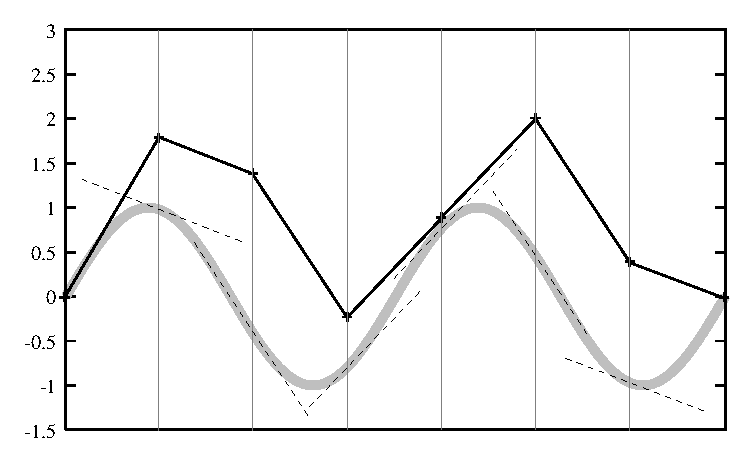
\includegraphics{figures/euler}}
\caption{Demonstration of Euler's method for solving the ODE of simple harmonic oscillation.
    The broad grey line represents the exact solution. At each time step, the method takes the
    derivative (gradient) of the function and uses it to extrapolate linearly.\label{eulersMethod}}
\end{figure}

The general scheme for numerical ODE solvers is to take the value of a function $f(t')$ and its
derivative $\frac{\diff f}{\diff t}(t')$ at some point in time $t'$. From these the algorithm
extrapolates what the value of the function is expected to be some time step $h$ later. The
simplest, most frequently-quoted and worst algorithm for this purpose is Euler's method,
\begin{equation}
f(t'+h) = f(t') + h\frac{\diff f}{\diff t}(t'),
\end{equation}
which performs linear extrapolation. Figure~\ref{eulersMethod} illustrates its operation. The
errors become smaller for tiny time steps, but the method still has a tendency of gaining energy
and is therefore unreliable.

\section{Quaternions\label{quaternions}}
\subsection{The need for Quaternions}
Besides its position, every rigid body in 3D space may have an orientation, in which there are
three degrees of freedom (three independent axes to rotate about).
While the position of a body can be neatly represented using Cartesian coordinates, there is
no obvious best way of describing an orientation. The most common schemes describe
it in terms of a rotation operation which transforms a vector in the body's local
coordinates into world coordinates (or \textsl{vice versa}). But again, there are various different
approaches to representing this rotation, all of which have advantages and disadvantages.

\emph{Euler angles} are probably the most intuitive representation of a 3D rotation, describing
it as a series of three rotations about different axes. These axes are fixed by convention, so it
suffices to specify the three angles of rotation. However, this scheme has a number of
drawbacks~\cite{Saunders:PhD,Shoemake:85}: amongst other things, it is possible that rotation
about one of the axes freezes during an animation (``Gimbal lock'').

\emph{Rotation matrices} are commonly used because they are well understood, easily generalize
to higher dimensions and allow efficient combination with other linear transformations (scaling
and shearing~-- also translation if homogeneous coordinates are employed). However, ODEs over
rotation matrices are difficult to implement correctly, since this representation uses nine
numbers (a $3\times3$ matrix) to represent three degrees of freedom, thus introducing six
additional side conditions which must be maintained. Not doing so causes skew through numerical
drift~\cite{Saunders:PhD}.

\emph{Quaternions}~\cite{Shoemake:85,Eberly:01,MathWorld:Quaternion} are a popular alternative
to the two previous schemes, and they are used extensively in this project.

\subsection{Definition and properties}
Mathematically, quaternions can be regarded as numbers with one real part and three
distinct imaginary parts:
\begin{equation}
\q{q} = q_w + q_x\qi + q_y\qj + q_z\qk
\end{equation}
where $q_w$, $q_x$, $q_y$ and $q_z$ are real numbers and \qi{}, \qj{} and \qk{} satisfy
\begin{equation}
\qi^2 = \qj^2 = \qk^2 = \qi\qj\qk = -1.
\end{equation}
From this follows that
$\qi\qj = -\qj\qi = \qk$ and
$\qj\qk = -\qk\qj = \qi$ and
$\qk\qi = -\qi\qk = \qj$.
Note that multiplication is not commutative.

We will also need the conjugate and the inverse of a quaternion. In analogy to
complex numbers, these are given respectively by
\begin{eqnarray}
\overline{\q{q}} & = & q_w - q_x\qi - q_y\qj - q_z\qk\\
\q{q}^{-1} & = & \frac{\overline{\q{q}}}{\norm{\q{q}}^2}\\
\mathrm{where}\quad&& \norm{q_w + q_x\qi + q_y\qj + q_z\qk} =
    \sqrt{q_w^2 + q_x^2 + q_y^2 + q_z^2}
\end{eqnarray}

Sometimes we will need to relate a 3D vector to a quaternion with zero real part.
For a given vector $\ve{u} = (u_1, u_2, u_3)^T$ we define the corresponding
quaternion to be
\begin{equation}
\label{vectorToQuat}
\tilde{\ve{u}} = u_1\qi + u_2\qj + u_3\qk.
\end{equation}

The complex constants \qi{}, \qj{} and \qk{} are required for the algebra
only, therefore we can represent a quaternion as four numbers $(w,x,y,z)$. It turns out that a
quaternion with unit magnitude ($\norm{\q{q}} = 1$) neatly represents an arbitrary rotation in
3D space, similarly to the way that an ordinary complex number represents a rotation in the 2D
Argand diagram. The condition $\norm{\q{q}} = 1$ reduces the number of degrees of freedom to
three, as required.

Every unit quaternion represents a rotation of angle $\theta$ about an arbitrary axis.
If the axis passes through the origin and has a direction given by the vector
\ve{a} with $\norm{\ve{a}} = 1$, the quaternion describing this rotation is
\begin{equation}
\label{quatRotation}
\q{q} = \cos\left(\frac{\theta}{2}\right) + \tilde{\ve{a}} \sin\left(\frac{\theta}{2}\right).
\end{equation}
It can easily be verified that this quaternion always has unit magnitude. It shall be assumed
throughout this project that the rotation thus described is clockwise (as seen when looking in
the direction of the vector $\ve{a}$) in a right-hand coordinate system, i.e.\ that it is
given by the ``right-hand rule''.

Two rotations can be concatenated by multiplying their quaternions together. The order in which
these rotations are applied is significant, and quaternion multiplication is not commutative,
so the semantics match. The operations are, however, associative. The quaternion product is
obtained simply by multiplying out the components, observing the rules for multiplying \qi{},
\qj{} and \qk{}:
\begin{eqnarray}
\lefteqn{(p_w + p_x\qi + p_y\qj + p_z\qk)(q_w + q_x\qi + q_y\qj + q_z\qk) = } \nonumber\\*
&& (p_w q_w - p_x q_x - p_y q_y - p_z q_z) + 
   (p_w q_x + p_x q_w + p_y q_z - p_z q_y) \,\qi + \nonumber\\*
&& (p_w q_y + p_y q_w + p_z q_x - p_x q_z) \,\qj + 
   (p_w q_z + p_z q_w + p_x q_y - p_y q_x) \,\qk \label{quatProduct}
\end{eqnarray}

To rotate a vector $\ve{v} = (v_1, v_2, v_3)^T$ by a quaternion \q{q}, we first
convert it into its corresponding quaternion $\tilde{\ve{v}}$ as defined in
equation~\ref{vectorToQuat} and then calculate the quaternion product
\begin{equation}
\label{quatTransform}
\tilde{\ve{v}}' = \q{q}\tilde{\ve{v}}\q{q}^{-1}
\end{equation}

If we expand this formula, we find that the real part of the result is always zero, and
that the rotated vector $\ve{v}' = (v_1', v_2', v_3')^T$ corresponds
to $\tilde{\ve{v}}'$ (i.e.\ $\ve{v}'$ is contained in the three complex parts of
the quaternion product).

Some authors, notably Shoemake~\cite{Shoemake:85}, choose to define the product in
equation~\ref{quatTransform} in
the reverse order. The choice is a matter of convention, since it merely changes the effect
of this operation from being a clockwise to a counter-clockwise rotation. I chose the clockwise
convention because it is consistent with the usual definition of the angular velocity vector
in physics.

Observe that under this convention, if \q{q} is itself a product of quaternions
$\q{q} = \q{q}_n \q{q}_{n-1} \cdots \q{q}_1$, the result is that of first applying the
$\q{q}_1$ rotation, then $\q{q}_2$ etc. In other words, the rotations in a quaternion product
are applied from right to left. To verify that this is the case, the identity
$\overline{\q{p}\, \q{q}} = \q{\overline{q}}\; \q{\overline{p}}$
is useful~\cite{MathWorld:Quaternion}.

\subsection{Quaternion integration}

We have seen that given the torques on a body, a numerical ODE solver can treat each component
of the vector separately to obtain the new angular momentum. Now that we are representing
orientation as a quaternion, how do we compute the change in orientation given the body's angular
velocity?

The instantaneous rate of change of a quaternion \q{q} over time is
usually~\cite{BaraffWitkin:97,Eberly:04,Saunders:PhD} given as
\begin{equation}
\label{quatRateOfChange}
\dot{\q{q}}(t) = \frac{1}{2}\tilde{\ve{\omega}}(t)\q{q}(t)
\end{equation}
where $\tilde{\ve{\omega}}$ is the quaternion corresponding to the angular velocity
vector $\ve{\omega}$. The quaternion $\dot{\q{q}}$ can be fed into an ODE solver which can handle
its four components separately. However, when this is done it is observed that the new orientation
$\q{q}'$ no longer has unit magnitude. This is an inherent property of the definition in
equation~\ref{quatRateOfChange}, and not, as sometimes claimed~\cite{Eberly:04}, merely a matter
of numerical round-off (proof in appendix~\ref{quatIntegrationMagnitude}). Usually this problem
is `solved' by normalizing the quaternion:
\begin{equation}
\q{q}(t + h) = \frac{\q{q}'}{\norm{\q{q}'}} \quad\quad\mathrm{where}\quad
    \q{q}' = \q{q}(t) + h\dot{\q{q}}(t)
\end{equation}
(using Euler's method for clarity; $\q{q}'$ would be appropriately redefined when using e.g.\ RK4).
This `solution' seemed quite \textsl{ad hoc} to me, and I indeed showed that it returns a
completely wrong result if the angular velocity is large (see appendix~\ref{quatNormalization}).

To obtain the correct result, the ODE solver must be modified. Whenever it calculates the sum of
a quaternion and a scaled derivative, as in $\q{q}(t) + h\dot{\q{q}}(t)$, we replace the summation
by $\mathrm{Quergs}(\q{q}(t), h\dot{\q{q}}(t))$, where $\mathrm{Quergs}$ is the
\emph{Qu}at\emph{er}nion inte\emph{g}ration \emph{s}tep\footnote{This naming follows the spirit of
Shoemake~\cite{Shoemake:85}, whose ``Slerp'' function is an `acronym' of \emph{S}pherical
\emph{l}inear int\emph{erp}olation.}:
\begin{equation}
\label{quergs}
\mathrm{Quergs}(\q{q}, \Delta\q{q}) =
    \frac{\q{q} + \tan\left(\norm{\Delta\q{q}}\right)
        \frac{\Delta\q{q}}{\norm{\Delta\q{q}}}}{
    \sqrt{\norm{\q{q}}^2 + \tan^2\left(\norm{\Delta\q{q}}\right)}}
\end{equation}

This formula is derived in appendix~\ref{quatIntegrationDerivation} and applied to the RK4
algorithm in appendix~\ref{quergsRK4}. It ensures that the resulting quaternion has unit magnitude
and is correct even at high velocities. I have not come across anything like it in the literature
I have searched, and hence have some grounds to believe it may be new.

\section{Constrained rigid body dynamics}
The methods we have developed so far allow the simulation of a single rigid body with forces
acting on it. Further challenges arise when we consider multibody systems in which the bodies
interact in some way. We will primarily be interested in articulated bodies, that is, systems
of individual rigid bodies held together by joints. Joints allow rotation but cannot be
separated. (The human body is a good example of such an articulated body.)

There are various strategies for implementing articulated bodies. {\em Lagrangian mechanics}
is a commonplace method in physics and engineering, in which the state of the system is expressed
in terms of a set of {\em generalised coordinates}. The position and orientation of each sub-body
is then a function of these generalised coordinates, and outside forces can be transformed
back into the generalised coordinates, where they are handled. For example, consider two rigid
bodies which are held together by a ball-and-socket joint~\cite{Kalra:95}. Without the joint,
the system would have 12 degrees of freedom at rest: three translational and three rotational
degrees for each of the bodies. In a Lagrangian formulation, the two connected bodies would be
expressed in nine coordinates: six for translation and rotation of the first body, and three
for the rotation of the second body with respect to the first.

Lagrangian mechanics has the advantage that if formulated correctly, the system will always in a
legal state, no matter what the values of the coordinates are. It also allows very fast
computation. On the downside, the functions to transform the coordinates become very hard or
impossible to find for complicated systems, so the method does not scale well.

An alternative approach to the problem is to initially grant each sub-body its full number of
degrees of freedom, and then to impose constraints on the system. We can then ensure that the
constraints are always maintained by excerting appropriate forces and torques on the bodies.
Finding these forces is commonly done by means of {\em Lagrange multipliers}~-- note that
despite the similarity in name, this method has very little in common with Lagrangian mechanics.

Lagrange multipliers are used to implement constrained rigid body mechanics in this project,
because once set up, such a system can handle a large variety of situations with ease.
The mathematical formulation of Lagrange multipliers is derived in~\cite{BaraffWitkin:97} and
extended in~\cite{Saunders:PhD} (also see~\cite{Baraff:96} for an optimized algorithm),
therefore we only state the results here.

Consider a system of $n$ rigid bodies at a particular point in time. Each body has a vector
pointing to its centre of mass, and an orientation. Assume that we can concatenate these
parameters of all bodies into a global state vector\footnote{Witkin calls this vector
$\ve{q}$; we use $\ve{x}$ here to avoid confusion with quaternions.} $\ve{x}$.
Containing a value for each degree of freedom, $\ve{x}$ will have $6n$ rows. In practice
we will never need to write down $\ve{x}$ explicitly; instead we will work with its
first and second derivative in time, $\dot{\ve{x}}$ and $\ddot{\ve{x}}$ respectively.

For example, in a system with two bodies, having centre of mass positions $\ve{a}$ and
$\ve{b}$, and angular velocities $\ve{\omega}$ and $\ve{\phi}$ respectively, we would
have
\begin{equation}
\label{lagrangeStateVector}
\dot{\ve{x}} = \left[ \begin{array}{c}
    \dot{\ve{a}}\\ \ve{\omega}\\ \dot{\ve{b}}\\ \ve{\phi} \end{array}\right]
\quad\quad\mathrm{and}\quad\quad
\ddot{\ve{x}} = \left[ \begin{array}{c}
    \ddot{\ve{a}}\\ \dot{\ve{\omega}}\\ \ddot{\ve{b}}\\ \dot{\ve{\phi}} \end{array}\right]
\end{equation}

Now assume that we want to impose $m$ constraints on this system, where each constraint
effectively reduces the number of degrees of freedom by one. (A constraint specifying a
ball-and-socket joint, as described earlier, would therefore have to be expressed as a
vector of three constraints.) Express each constraint as a function $c$ which is zero
when the constraint is satisfied. We can then combine all constraint functions into a
single $m$-row constraint vector $\ve{c}$. Each valid configuration of the system must
satisfy $\ve{c} = \ve{0}$, the null vector.

To find the constraint maintaining forces, we must know how a change in state or a change in
time affects the value of $\ve{c}$. To this end, we must calculate the first two partial
derivatives of $\ve{c}$ with respect to time, $\dot{\ve{c}}$ and $\ddot{\ve{c}}$.
We also calculate the Jacobian matrix~\cite{RHB:02} $\m{J}$ which contains all partial
derivatives of $\ve{c}$ w.r.t. all coordinates of $\ve{c}$, and the similarly
defined Jacobian $\dot{\m{J}}$ of $\dot{\ve{c}}$:
\begin{equation}
J_{ij} = \frac{\partial c_i}{\partial x_j} \quad\quad\mathrm{and}\quad\quad
\dot{J}_{ij} = \frac{\partial \dot{c}_i}{\partial x_j}
\end{equation}

Both $\m{J}$ and $\dot{\m{J}}$ are $6n\times m$ matrices. However, since we do not
have an explicit expression for $\ve{x}$, we cannot calculate them directly using
partial differentiation. Instead we make use of the following results of the chain rule:
\begin{equation}
\label{cDotAndCDDot}
\dot{\ve{c}} = \m{J}\dot{\ve{x}} \quad\quad\mathrm{and}\quad\quad
\ddot{\ve{c}} = \dot{\m{J}}\dot{\ve{x}} + \m{J}\ddot{\ve{x}}.
\end{equation}
Appendix~\ref{constraintAppendix} gives examples of derivations using these equations.

Two more quantities are required before we can determine the forces and torques which maintain
our constraints. We need to add up all the other forces and torques acting on each of the $n$
sub-bodies (for example due to gravity or muscular activity) and concatenate them into a single
$6n$-row vector \ve{\Phi}, just as we did for \ve{x}. Re-using the two-body case of
equation~\ref{lagrangeStateVector}:
\begin{equation}
\ve{\Phi} = \left[\begin{array}{l}
    \sum \ve{F}_A \\
    \left( \sum \ve{\tau}_A \right) - \ve{\omega}\times(\m{I}_A\,\ve{\omega}) \\
    \sum \ve{F}_B \\
    \left( \sum \ve{\tau}_B \right) - \ve{\phi}\times(\m{I}_B\,\ve{\phi})
    \end{array}\right]
\end{equation}
where $\ve{F}_A$ denotes a force vector acting on the centre of mass of body~A, $\ve{\tau}_A$
is a torque vector acting on body~A, and $\m{I}_A$
the moment of inertia of body~A in the world frame. The expression
$\ve{\omega}\times(\m{I}_A\,\ve{\omega})$ and its analogue for the other bodies do
not strictly represent torques, but subtracting them here ensures that angular momentum is
conserved in the absence of other torques. See appendix~\ref{correctBrettAppendix} for the
derivation of this expression.

And finally, we require the {\em mass-inertia tensor} \m{M} and its inverse
$\m{M}^{-1}$. Both are $6n\times6n$ matrices of the form
\begin{equation}
\label{massInertiaTensor}
\m{M} = \left[ \begin{array}{ccccccc}
    \mu_1\m{1} \\ & \m{I}_1 \\ &&
    \mu_2\m{1} \\ &&& \m{I}_2 \\ &&&& \ddots \\ &&&&&
    \mu_n\m{1} \\ &&&&&& \m{I}_n
    \end{array}\right]
\end{equation}

Here $\mu_i$ denotes the (scalar) mass of body $i$, \m{1} stands for the $3\times3$
identity matrix, and $\m{I}_i$ is the inertia tensor (written as a $3\times3$ matrix)
of body $i$ in the world frame. All empty regions are zero. While $\mu_i$ will typically
stay constant over time, $\m{I}_i$ may depend on the orientation of body $i$.\footnote{If
we know the principal axes of the body, we can express \m{I} in a time-invariant
form combined with rotations into the principal axes frame and back again
(see~\cite{BaraffWitkin:97}), which saves us a lot of effort.} The inverse $\m{M}^{-1}$
is obtained by replacing each $\mu$ by $\frac{1}{\mu}$ and each $\m{I}$ by
$\m{I}^{-1}$ in equation~\ref{massInertiaTensor}.

Now we can set up the equation\footnote{Here we adopt the sign convention
of~\cite{BaraffWitkin:97}, which is the opposite of~\cite{Saunders:PhD}.}
\begin{equation}
\label{lagrangeEquation}
-\m{J}\m{M}^{-1}\m{J}^T\ve{\lambda} = \dot{\m{J}}\dot{\ve{x}} +
    \m{J}\m{M}^{-1}\ve{\Phi} + k\ve{c} + d\dot{\ve{c}}
\end{equation}
in which all variables except $\ve{\lambda}$ are known. The meaning of this equation and
its two scalar constants $k$ and $d$ is discussed in~\cite{BaraffWitkin:97}
and~\cite{Saunders:PhD}. For us it will suffice to consider it to be a `black box' which can be
given to a linear equation solver to obtain $\ve{\lambda}$.

$\ve{\lambda}$ is an $m$-row vector of so-called Lagrange multipliers (after which this method
is named), where $m$ is the number of constraints. Once we have solved for it, we can compute
the expression
\begin{equation}
\hat{\ve{\Phi}} = \m{J}^T\,\ve{\lambda}.
\end{equation}
$\hat{\ve{\Phi}}$ has the same format as $\ve{\Phi}$, and indeed it is the vector containing
the forces and torques which we need to additionally apply to each body to ensure that they
continue to satisfy the constraints! The bodies' constrained movements are calculated by
the generalised form of the familiar formula $\ddot{x} = \frac{F}{m}$:
\begin{equation}
\ddot{\ve{x}} = \m{M}^{-1}\,(\ve{\Phi} + \hat{\ve{\Phi}})
\end{equation}
This result, $\ddot{\ve{x}}$, can now be fed directly into our ODE solver.

\section{Collision and contact}

We now have all the mathematical facilities we need to simulate mechanical systems in which
the acceleration functions are continuous over time. This already covers a large number of
interesting systems, but unfortunately excludes any sort of collision between bodies. If we want
to examine systems of separable but non-penetrating bodies, we have to open a whole new can of
worms.

Let us distinguish two cases of contact between bodies: resting contact and colliding contact.
A book lying on your desk is in resting contact with the surface: their relative velocity is zero,
but the desk excerts a force on the book to prevent it from penetrating into the surface.
Colliding contact is given for example between the ground and a ball bouncing off it. In real
life, the ball stays in contact with the ground for a finite length of time, during which it is
deformed and experiences a finite force accelerating it upwards. In our simulation, however, we
are working with rigid bodies which cannot be deformed, so we want the collision to happen
instantaneously in the moment when the ball touches the ground. One way of looking at this is as
an infinitely strong force acting over an infinitely short time, but a more useful representation
is in terms of an impulse exchanged between the bodies.

Creating a simulation involving contacts is generally seen as a difficult task.
Baraff~\cite{BaraffWitkin:97} derives equations to handle collisions, and outlines (with a number
of errors) a way of handling resting contact. Unfortunately his collision handling does not work
in combination with constraints~-- it violates the assumption that the constraint function is
twice differentiable~-- and his resting contact computation relies on a complicated and uncommon
numerical routine. In this project, a new method of handling contacts is developed, which is
simpler to implement, more powerful, and works perfectly together with constraints like those
described in section~\ref{constraints}.

In the rest of this section we will examine the simulation only at one point in time, at which
the bodies in question are in contact. We also assume that we know the place at which the contact
occurs. Algorithms for finding both the time and place of contact are discussed elsewhere in this
report.

\subsection{Resting contact}

To keep things manageable, let us assume that we are dealing only with polyhedral bodies~-- bodies
whose exterior consists of flat polygon faces, delimited by vertices, joined by straight edges.
Since we will actually be working with a triangle mesh, this is fine.

There are two main ways in which polyhedra can be in contact: either by a vertex of one body being
inside a face of the other body, or by an edge of one body intersecting an edge of the other.
There remain a few corner cases, but we will think about those later. The book lying on your desk
may for example have four vertex/face contacts, each of the four corners of its back cover
touching the face of the desk surface. You may visualize edge/edge contacts by holding the book
such that its spine is touching the front edge of your desk.

In both cases, for the bodies not to interpenetrate, they must excert equal and opposite forces on
each other. This force must exactly balance the outside force, otherwise they would accelerate
apart. Also in both cases the direction of the force is perpendicular to the plane of contact. In
the vertex/face case, this plane is just the plane of the face polygon. In the edge/edge case, the
plane goes through the point of contact and is spanned by the directions of the two edges involved.
Modulo its sign, this plane's unit normal vector is unique~-- except if the two edges are
parallel, which is a case we will ignore for now.



\begin{appendix}
\chapter{Proofs and derivations}
All work presented in this appendix, unless otherwise specified, is the sole work
of the author and is not given in any of the literature which the author is aware of.
\section{Quaternion integration\label{quatProofs}}

Let us first consider a geometric view on quaternions, taken from~\cite{Shoemake:85}. Treat
the four components of a quaternion as Cartesian coordinates of a four-dimensional vector
space. The set of unit quaternions is then the surface of a unit hypersphere (also called a
\emph{glome}~\cite{MathWorld:4D}) in this vector space. Each point on this hypersphere
corresponds to a particular rotation. It also turns out that each pair of
opposite points on this sphere represent exactly the same rotation; hence all possible
rotations are contained in one hemisphere, no matter where the sphere is cut in half.

\subsection{Conservation of magnitude\label{quatIntegrationMagnitude}}
Define the quaternion dot product, in analogy to the 4D vector dot product, to be
\begin{equation}
\q{p}\cdot\q{q} =
    (p_w + p_x\qi + p_y\qj + p_z\qk)\cdot (q_w + q_x\qi + q_y\qj + q_z\qk) =
    p_w q_w + p_x q_x + p_y q_y + p_z q_z
\end{equation}
The dot product is commutative, contrary to the `standard' quaternion product.

The instantaneous rate of change is given~\cite{BaraffWitkin:97,Eberly:04,Saunders:PhD} to be
\begin{eqnarray*}
\dot{\q{q}} & = & \frac{1}{2}\ve{\omega}\q{q} =
    \frac{1}{2}(\omega_1\qi + \omega_2\qj + \omega_3\qk)
    (q_w + q_x\qi + q_y\qj + q_z\qk) \\*
& = & \frac{1}{2} ( - \omega_1 q_x - \omega_2 q_y - \omega_3 q_z ) +
    \frac{\qi}{2} ( \omega_1 q_w + \omega_2 q_z - \omega_3 q_y ) + \\*
&&  \frac{\qj}{2} (-\omega_1 q_z + \omega_2 q_w + \omega_3 q_x ) +
    \frac{\qk}{2} ( \omega_1 q_y - \omega_2 q_x + \omega_3 q_w )
\end{eqnarray*}

We now treat \q{q} and $\dot{\q{q}}$ as 4D vectors and calculate
their dot product:
\begin{eqnarray*}
\q{q}\cdot\dot{\q{q}} & = & \frac{1}{2} (
    - q_w \omega_1 q_x - q_w \omega_2 q_y - q_w \omega_3 q_z
    + q_x \omega_1 q_w + q_x \omega_2 q_z - q_x \omega_3 q_y \\*
&&  - q_y \omega_1 q_z + q_y \omega_2 q_w + q_y \omega_3 q_x
    + q_z \omega_1 q_y - q_z \omega_2 q_x + q_z \omega_3 q_w ) \\*
& = & 0.
\end{eqnarray*}
The rate of change is orthogonal to \q{q}, and therefore it is always
a tangent to the sphere, touching it at the point corresponding to \q{q}. The set of all possible
values of $\dot{\q{q}}$ is thus a hyperplane (a three-dimensional subspace) tangential to the
sphere at the point \q{q} in 4D space.

We can determine the magnitude $\norm{\dot{\q{q}}}$ from the sum of squares of the
components given above and find it to be
$\norm{\dot{\q{q}}} = \frac{1}{2}\norm{\ve{\omega}}\,\norm{\q{q}}$. Since we always
require $\q{q}$ to be a unit quaternion, we can reduce this to
\begin{equation}
\label{quatRateOfChangeMagnitude}
\norm{\dot{\q{q}}} = \frac{1}{2}\norm{\ve{\omega}}.
\end{equation}

Now let us determine what happens if we calculate $\q{q} + h\dot{\q{q}}$ for some finite $h$.
Note that this operation is required by all common numerical solvers of differential equations.
Consider the magnitude of the result:
\begin{eqnarray*}
\norm{\q{q} + h\dot{\q{q}}}^2 & = & (\q{q} + h\dot{\q{q}})\cdot(\q{q} + h\dot{\q{q}}) \\
&=& \q{q}\cdot\q{q} + 2h\q{q}\cdot\dot{\q{q}} + h^2\dot{\q{q}}\cdot\dot{\q{q}} \\
&=& 1 + 0 + \frac{h^2}{4}\norm{\ve{\omega}}^2 \\
&>& 1 \quad\quad\mbox{whenever}\quad \norm{\ve{\omega}} > 0.
\end{eqnarray*}

Hence, if the body in question is rotating, it is not possible for a standard numerical ODE solver
to preserve a quaternion's property of unit magnitude.


\subsection{Normalization is not enough\label{quatNormalization}}

One should think that given the derivative of a quaternion \q{q} (equation~\ref{quatRateOfChange},
page~\pageref{quatRateOfChange}) that we can find $\q{q}(t + h)$ for some time step $h$ within
the accuracy of the ODE solver employed ($O(h^5)$ error for fourth-order Runge-Kutta).
Unfortunately this is not the case. This shall be demonstrated using Euler's method; it should,
however, be pointed out that more sophisticated methods like RK4 are also affected. Consider the
value of \q{q} at the next time step, $\q{q}(t + h) = \q{q}(t) + h \dot{\q{q}}(t)$. For any
non-zero $h$ and $\dot{\q{q}}$ this point will always lie outside the unit quaternion sphere due
to the orthogonality of \q{q} and $\dot{\q{q}}$. This is usually compensated by re-normalizing
the quaternion after the ODE solving step. Geometrically, this re-normalization can be understood
as drawing a straight line through the origin and the point $\q{q}(t) + h \dot{\q{q}}(t)$,
intersecting this line with the unit sphere and replacing $\q{q}(t + h)$ by this point of
intersection (see figure~\ref{quatNormalizationFigure}).

\begin{figure}
\psfrag{frag:q}{\q{q}}
\psfrag{frag:qdot}{$\dot{\q{q}}$}
\psfrag{frag:qplusqdot}{$\q{q} + h\dot{\q{q}}$}
\centerline{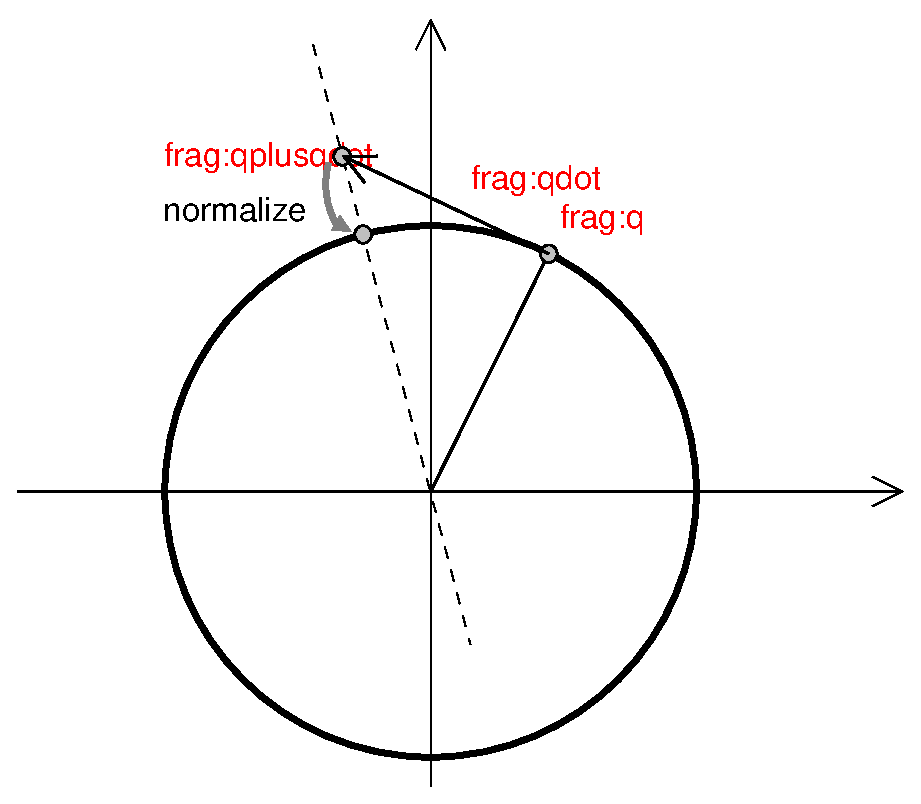
\includegraphics[width=6cm]{figures/quaternion1}}
\caption{Normalizing a quaternion after performing an ODE solving step.
    \label{quatNormalizationFigure}}
\end{figure}

Following the tangent to the sphere is a reasonable approximation to following its curve if the
magnitude of $h \dot{\q{q}}(t)$ is small compared to the curvature of the sphere.
For large time steps or large magnitudes of \ve{\omega}, however, this gets increasingly
erroneous. Consider the limiting case, a body rotating infinitely fast
($\norm{\ve{\omega}} \rightarrow \infty$): after re-normalisation, $\q{q}$ will have moved merely
a quarter of the way around the unit sphere, which equates to concatenating the rotation of
quaternion \q{q} with a rotation by $180^\circ$. This is a strictly finite amount of rotation
per time step, while it would actually have been correct to perform an infinite number of
revolutions around the quaternion sphere.

If a polynomial approximation method like RK4 had been used instead of Euler's method, a
polynomial space curve would have been fitted to the surface of the sphere instead of a straight
line. Note however that the Taylor series of the $\sin$ and $\cos$ functions are nonterminating,
and that it is therefore not possible for a finite polynomial curve to lie exactly in the surface
of a sphere. These ODE solvers will therefore suffer the same problems, albeit less pronounced.


\subsection{Corrected quaternion integration\label{quatIntegrationDerivation}}

Assume that the body we are simulating is rotating at a constant angular velocity.
(This assumption is later weakened by the use of a more sophisticated ODE solver,
but for now we will stick with Euler's method.) Furthermore assume without loss of
generality that the body is rotating clockwise about its $x$ axis, which corresponds
to the world's $x$ axis, and that at time $t=0$ the body's frame and the world frame
coincide. Then the orientation of the body (the quaternion describing
the linear transformation to get from the body's frame of reference into the world
frame) is given as a function of time by
\begin{equation}
\label{quatDerivationExact}
\q{q}(t) = \cos\left(\frac{\norm{\ve{\omega}}t}{2}\right) +
    \sin\left(\frac{\norm{\ve{\omega}}t}{2}\right)\qi
\end{equation}
(cf.\ equation~\ref{quatRotation}, figure~\ref{quatIntFig1}) and its angular velocity is
\begin{equation}
\ve{\omega} = (\omega_1, \omega_2, \omega_3)^T = (\norm{\ve{\omega}}, 0, 0)^T
\end{equation}
for some arbitrary $\norm{\ve{\omega}}$, measured in radians per unit time.

\begin{figure}
\psfrag{frag:omegat}{$\frac{\norm{\ve{\omega}} t}{2}$}
\psfrag{frag:qdotoft}{$\dot{\q{q}}(t)$}
\psfrag{frag:real}{Re}
\psfrag{frag:iimag}{i-Im}
\centerline{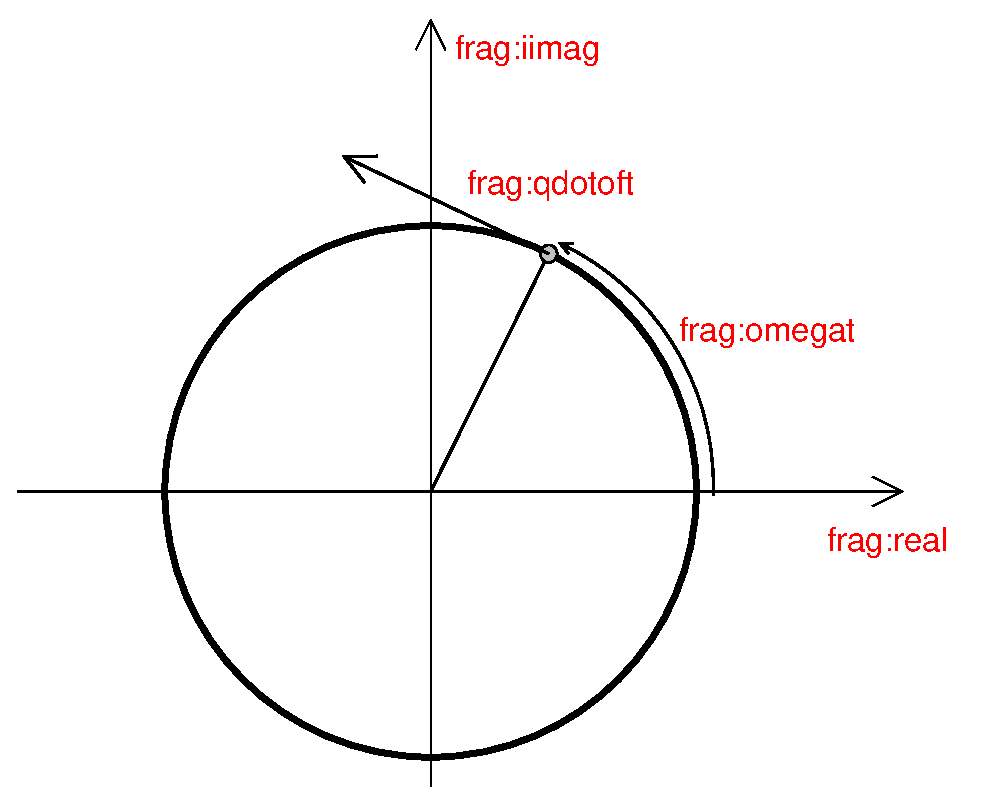
\includegraphics[width=6cm]{figures/quaternion2}}
\caption{Assumed situation for the derivation in
section~\ref{quatIntegrationDerivation}.\label{quatIntFig1}}
\end{figure}

Now assume w.l.o.g.\ that we take a time step from $t = 0$ to $t = h$.
Then we require that the result returned by Euler's method for $\q{q}(h)$
after re-normalization be equal to its exact value in equation~\ref{quatDerivationExact}:
\begin{equation}
\label{quatDerivationSetup}
\cos\left(\frac{\norm{\ve{\omega}} h}{2}\right) +
    \sin\left(\frac{\norm{\ve{\omega}} h}{2}\right)\qi =
    \frac{\q{q}(0) + h \dot{\q{q}}(0)}
        {\norm{\q{q}(0) + h \dot{\q{q}}(0)}}
\end{equation}

We know from examining the 4D geometry that the value assigned to $\dot{\q{q}}$
in equation~\ref{quatRateOfChange} has the correct direction and merely needs to be
corrected in magnitude. In other words, we are searching for a scalar function
$f(h, \norm{\ve{\omega}})$ which will allow $\dot{\q{q}}$ to satisfy
equation~\ref{quatDerivationSetup}:
\begin{equation}
\dot{\q{q}}_h(t) = f\tilde{\ve{\omega}}(t)\q{q}(t)
\end{equation}

Observe that under the above assumptions $\q{q}(0) = 1$, and thus
$\dot{\q{q}}_h(0) = f \norm{\ve{\omega}} \qi$. Substituting this
into equation~\ref{quatDerivationSetup} and considering only the real part:
\begin{eqnarray*}
&& \cos\left(\frac{\norm{\ve{\omega}} h}{2}\right) =
    \left[1 + \left( f \norm{\ve{\omega}} h \right)^2 \right]^{-\frac{1}{2}} \\
&\Leftrightarrow&
    \left( f \norm{\ve{\omega}} h \right)^2 =
    \frac{1}{\cos^2\left(\frac{\norm{\ve{\omega}} h}{2}\right)} - 1 \\
&\Leftrightarrow&
    f(h, \norm{\ve{\omega}}) =
    \frac{1}{\norm{\ve{\omega}} h} \sqrt{\frac{
        1 - \cos^2\left(\frac{\norm{\ve{\omega}} h}{2}\right)}{
        \cos^2\left(\frac{\norm{\ve{\omega}} h}{2}\right)}} =
    \frac{1}{\norm{\ve{\omega}} h}
        \tan\left(\frac{\norm{\ve{\omega}} h}{2}\right)
\end{eqnarray*}

To check, we substitute this result into the $\qi$-imaginary part of
equation~\ref{quatDerivationSetup}:
\begin{eqnarray*}
\sin\left(\frac{\norm{\ve{\omega}} h}{2}\right) & = &
    \tan\left(\frac{\norm{\ve{\omega}} h}{2}\right)
    \left[ 1 + \tan^2\left(\frac{\norm{\ve{\omega}} h}{2}\right)
    \right]^{-\frac{1}{2}} \\
&=& \tan\left(\frac{\norm{\ve{\omega}} h}{2}\right)
    \left[ \frac{\cos^2\left(\frac{\norm{\ve{\omega}} h}{2}\right) +
    \sin^2\left(\frac{\norm{\ve{\omega}} h}{2}\right) }{
    \cos^2\left(\frac{\norm{\ve{\omega}} h}{2}\right) }
    \right]^{-\frac{1}{2}} \\
&=& \tan\left(\frac{\norm{\ve{\omega}} h}{2}\right)
    \cos\left(\frac{\norm{\ve{\omega}} h}{2}\right) \\
&=& \sin\left(\frac{\norm{\ve{\omega}} h}{2}\right)
\end{eqnarray*}

Thus we establish the validity of this expression for $f$. Observe that by using 
L'Hospital's rule, we can find value of $f$ for an infinitesimally small time step:
$$
\lim_{h \to 0} f = \lim_{h \to 0} \frac{ \frac{\norm{\ve{\omega}}}{2}
    \cos^{-2}\left(\frac{\norm{\ve{\omega}} h}{2}\right) }{ \norm{\ve{\omega}} } =
    \frac{1}{2}
$$
i.e.\ we obtain the original equation~\ref{quatRateOfChange} for the
instantaneous rate of change.

Now let $\Delta \q{q} = h \dot{\q{q}} =
    \frac{h}{2} \tilde{\ve{\omega}} \q{q}$.
From equation~\ref{quatRateOfChangeMagnitude} we find that
$\norm{\Delta\q{q}} = \frac{\norm{\ve{\omega}} h}{2}$.
Hence we can simplify the expression for the quaternion correcting factor by expressing it
in terms of $\Delta \q{q}$ as follows:
$$
h f \tilde{\ve{\omega}}\q{q} = \frac{h}{\norm{\ve{\omega}} h}
    \tan\left(\frac{\norm{\ve{\omega}} h}{2}\right) \tilde{\ve{\omega}} \q{q} =
    \tan\left(\norm{\Delta\q{q}}\right) \frac{\Delta\q{q}}{\norm{\Delta\q{q}}}
$$

This expression now has a clear geometric interpretation with respect to the 4D geometry
(see figure~\ref{quatIntFig2}):
$\norm{\Delta\q{q}}$ is measured in radians, and it corresponds to the \emph{correct}
angle between the old and the new vector $\q{q}$. Since $\q{q}$ and
$\dot{\q{q}}$ are orthogonal, we have a right-angled triangle between the origin,
the old and the new points $\q{q}$, and hence we can use the $\tan$ function to
evaluate the required length of the side in direction $\Delta\q{q}$.

\begin{figure}
\psfrag{frag:real}{Re}
\psfrag{frag:iimag}{i-Im}
\psfrag{frag:q}{\q{q}}
\psfrag{frag:deltaq}{$\Delta\q{q}$}
\psfrag{frag:quergs1}{$\q{q}+\tan(\norm{\Delta\q{q}})\frac{\Delta\q{q}}{\norm{\Delta\q{q}}}$}
\psfrag{frag:quergs2}{$\mathrm{Quergs}(\q{q},\,\Delta\q{q})$}
\centerline{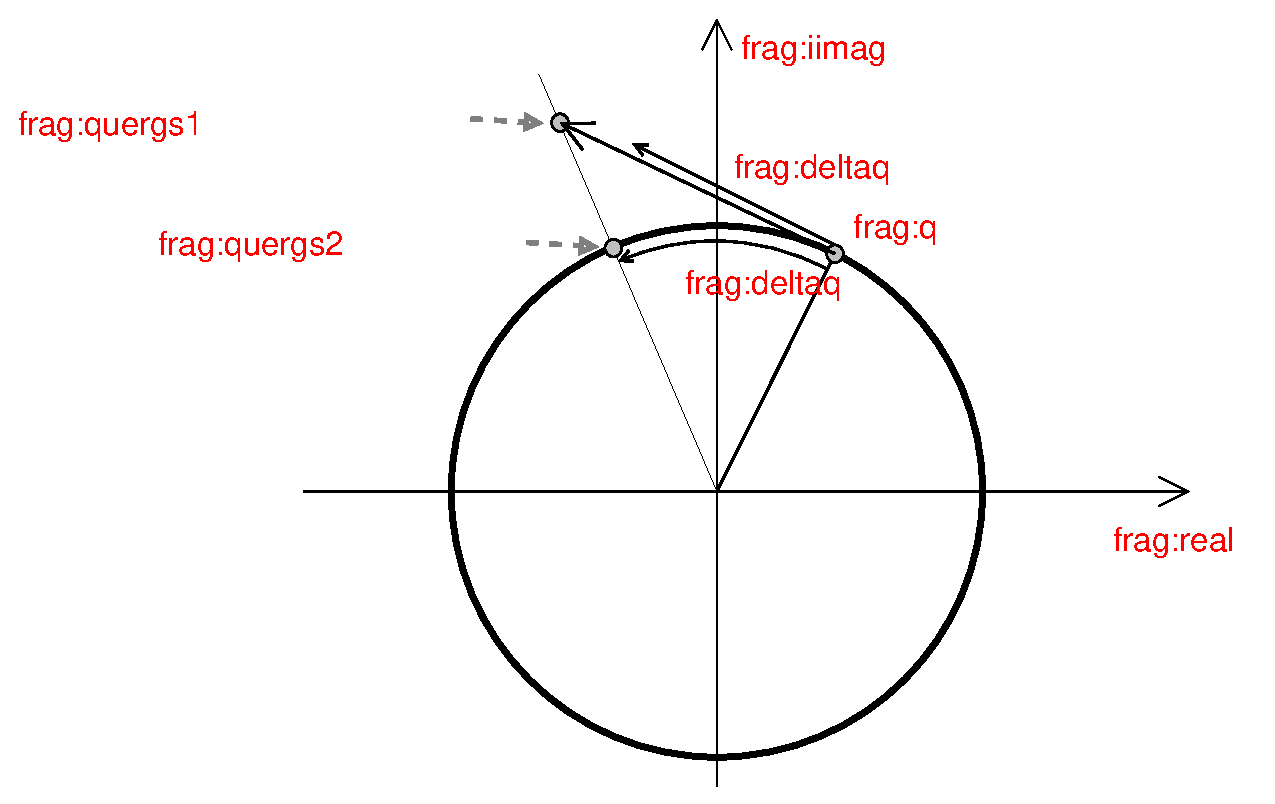
\includegraphics[width=7.7cm]{figures/quaternion3}}
\caption{Illustration of the operation of Quergs.\label{quatIntFig2}}
\end{figure}

Finally we can combine this correction and the subsequent quaternion normalisation into
a single function:
\begin{eqnarray*}
\q{q}(t+h) = \mathrm{Quergs}(\q{q}(t), \Delta\q{q}) &=&
    \frac{\q{q}(t) + \tan\left(\norm{\Delta\q{q}}\right)
        \frac{\Delta\q{q}}{\norm{\Delta\q{q}}}}{
    \norm{\q{q}(t) + \tan\left(\norm{\Delta\q{q}}\right)
        \frac{\Delta\q{q}}{\norm{\Delta\q{q}}}}} \\
&=& \frac{\q{q}(t) + \tan\left(\norm{\Delta\q{q}}\right)
        \frac{\Delta\q{q}}{\norm{\Delta\q{q}}}}{
    \sqrt{1 + \tan^2\left(\norm{\Delta\q{q}}\right)}} \\
&=& \left[\q{q}(t) + \tan\left(\norm{\Delta\q{q}}\right)
        \frac{\Delta\q{q}}{\norm{\Delta\q{q}}}\right]
    \cos\left(\norm{\Delta\q{q}}\right)
\end{eqnarray*}
The last expression is simplest (and again allows geometric interpretation), but probably
the first of the three expressions is more useful for numerical evaluation, since it involves
only one trigonometric function and minimizes numerical errors.

When implementing this formula, care must be taken around the discontinuities of the $\tan$
function, where numerical instability may occur. These discontinuities are reached whenever a
body performs an odd multiple of half revolutions during a single time step.


\subsection{Applying Quergs to Runge-Kutta\label{quergsRK4}}

Quergs implements one step of Euler's method for solving an ODE over a quaternion.
Where for Euler's method over an Euclidean vector we would write
$\ve{a}(t + h) = \ve{a}(t) + h\,\dot{\ve{a}}(t,\;\ve{a}(t))$,
for quaternions we simply use
$\q{q}(t + h) = \mathrm{Quergs}(\q{q}(t),\; h\,\dot{\q{q}}(t)) =
    \mathrm{Quergs}(\q{q}(t),\; \frac{h}{2}\,\tilde{\ve{\omega}}(t)\q{q}(t))$.

We can apply Quergs to polynomial ODE solvers by following the same pattern: wherever the solver
computes the sum of a quantity and a delta of that quantity (a delta being a derivative
scaled with the time step size and other factors), we substitute Quergs in place of that
addition. Assume we have a function $\dot{\q{q}}(t,\; \q{q}(t))$ which computes the
instantaneous rate of change at time $t$, given the state $\q{q}(t)$ at that time. Then we can
define the formulae for the fourth-order Runge-Kutta solver (RK4, based on the definition
in~\cite{NRinC}) over quaternions as follows:
\begin{eqnarray}
\Delta\q{q}_1 & = & h\;\dot{\q{q}}\left(t,\;\q{q}(t)\right) \nonumber\\
\Delta\q{q}_2 & = & h\;\dot{\q{q}}\left(t + \frac{h}{2},\;
    \mathrm{Quergs}\left(\q{q}(t),\; \frac{1}{2}\Delta\q{q}_1\right)\right) \nonumber\\
\Delta\q{q}_3 & = & h\;\dot{\q{q}}\left(t + \frac{h}{2},\;
    \mathrm{Quergs}\left(\q{q}(t),\; \frac{1}{2}\Delta\q{q}_2\right)\right) \nonumber\\
\Delta\q{q}_4 & = & h\;\dot{\q{q}}\left(t + h,\;
    \mathrm{Quergs}\left(\q{q}(t),\; \Delta\q{q}_3\right)\right) \nonumber\\
\q{q}(t + h) & = & \mathrm{Quergs}\left(\q{q}(t),\;
    \frac{1}{6}\Delta\q{q}_1 + \frac{1}{3}\Delta\q{q}_2 +
    \frac{1}{3}\Delta\q{q}_3 + \frac{1}{6}\Delta\q{q}_4\right)
\end{eqnarray}

Why is it correct to compute the weighted sum over $\Delta\q{q}_1$ to
$\Delta\q{q}_4$ in the last formula, when we have replaced all other quaternion additions
by calls to Quergs? Remember that finite movements on the quaternion hypersphere are
equivalent to rotations in 4D, and that these are not commutative. Differential
rotations are, however, commutative~-- like in 3D. (This is the reason why we can
use component-by-component integration to determine angular momentum:
like angular velocity, it is a differential of rotation.) Here, $\Delta\q{q}_1$ to
$\Delta\q{q}_4$ are also weighted differentials, and therefore subject to
conventional summation. Finally observe that each of $\Delta\q{q}_1$ to
$\Delta\q{q}_4$ is orthogonal to \q{q} (appendix~\ref{quatIntegrationMagnitude}),
and that therefore the weighted sum of all of these, expressed as a vector, also
lies in the hyperplane which is tangential to the unit sphere at the point \q{q},
and is therefore a valid derivative.

\section{Free precession\label{correctBrettAppendix}}

This argument is modelled after~\cite{Ruf:02}. The moment of inertia $\ve{L}$ of a rigid
body is defined as
\begin{equation}
\label{correctBrett1}
\ve{L} = \m{I}\ve{\omega}
\end{equation}
where $\m{I}$ is the inertia tensor and $\ve{\omega}$ is the angular velocity vector.
Torque is the rate of change of angular momentum over time:
\begin{equation}
\label{correctBrett2}
\ve{\tau} = \dot{\ve{L}} = \dot{\m{I}}\ve{\omega} + \m{I}\dot{\ve{\omega}}
\end{equation}

We can further evaluate $\dot{\m{I}}$ by writing \m{I} as a product with some rotation matrix
$\m{R}$ and its transpose:
\begin{equation}
\label{correctBrett3}
\m{I} = \m{R}\m{I}_\mathrm{body}\m{R}^T
\end{equation}

It can be shown that such a decomposition of the inertia tensor always exists, and that
$\m{I}_\mathrm{body}$ is a diagonal, time-invariant matrix containing the moments
of inertia about the body's principal axes~\cite{Feynman:63}. Hence we obtain
\begin{equation}
\label{correctBrett4}
\dot{\m{I}} = \dot{\m{R}}\m{I}_\mathrm{body}\m{R}^T +
    \m{R}\m{I}_\mathrm{body}\frac{\diff}{\diff t}\m{R}^T
\end{equation}

Witkin~\cite{BaraffWitkin:97} derives that $\dot{\m{R}} = \dual{\ve{\omega}}\,\m{R}$
for a rotation matrix $\m{R}$ and an angular velocity vector $\ve{\omega}$.
Using this identity and taking the differential operator onto the inside of the
transpose at the end of equation~\ref{correctBrett4},
\begin{eqnarray}
\dot{\m{I}} &=& \dual{\ve{\omega}}\,\m{R}\m{I}_\mathrm{body}\m{R}^T +
    \m{R}\m{I}_\mathrm{body}(\dual{\ve{\omega}}\,\m{R})^T \nonumber\\
&=& \dual{\ve{\omega}}\,\m{R}\m{I}_\mathrm{body}\m{R}^T -
    \m{R}\m{I}_\mathrm{body}\m{R}^T\dual{\ve{\omega}} \nonumber\\
&=& \dual{\ve{\omega}}\,\m{I} - \m{I}\dual{\ve{\omega}} \label{correctBrett5}
\end{eqnarray}

Substituting equation~\ref{correctBrett5} back into~\ref{correctBrett2}:
\begin{eqnarray}
\ve{\tau} & = & \m{I}\dot{\ve{\omega}} + \dual{\ve{\omega}}\,\m{I}\ve{\omega} -
    \m{I}\dual{\ve{\omega}}\,\ve{\omega} \nonumber \\
& = & \m{I}\dot{\ve{\omega}} + \dual{\ve{\omega}}\,\m{I}\ve{\omega} \label{correctBrett6}
\end{eqnarray}

Equation~\ref{correctBrett6} corrects the similar expression in~\cite{Saunders:PhD},
page~34. This means that the angular acceleration of a rigid body is given by
\begin{equation}
\label{correctBrett7}
\dot{\ve{\omega}} = \m{I}^{-1} (\ve{\tau} - \dual{\ve{\omega}}\,\m{I}\ve{\omega}).
\end{equation}
where \ve{\tau} is the sum of all torque vectors acting on the body. This means that even if
there are no torques, its angular velocity may change if \m{I} is not diagonal (i.e.\ if
the body is somehow asymmetric). This effect is called \emph{free precession}.

In a simulation, we usually integrate over torques to find angular momentum, and then calculate
the angular velocity from the momentum in each time step using the current moment of inertia. In
this case, the angular acceleration in equation~\ref{correctBrett7} is not needed. It is required
only for purposes of computing constraint forces and torques.

\section{A catalog of constraint functions\label{constraintAppendix}}

Let us consider some examples of constraints to clarify the procedure.

\subsection{Fixed point in space (`Nail')}

Let us implement a constraint which `nails' a particular point in a rigid body to a fixed point
in world space. (It's a very flexible nail, because despite fixing the position, it allows all
three modes of rotation.) Let \ve{p} be the position of the centre of mass of our rigid
body, \ve{s} the vector from the centre of mass to the point in the body we want to attach,
$\ve{\omega}$ the angular velocity of the rigid body, and \ve{t} the coordinates in world
space that we want to nail the point to. Then we can set up a very simple constraint function,
\begin{equation}
\ve{c} = \ve{p} + \ve{s} - \ve{t}
\end{equation}
which equals the null vector when $\ve{p}+\ve{s}$ and $\ve{t}$ coincide, as required.
Since this is a three-dimensional vector equation, we are actually defining three constraints
at once. Since \ve{t} does not change over time, we obtain
\begin{eqnarray}
\dot{\ve{c}} &=& \dot{\ve{p}} + \ve{\omega}\times\ve{s} \nonumber\\
&=& \dot{\ve{p}} - \dual{\ve{s}}\,\ve{\omega} \\
\ddot{\ve{c}} &=& \ddot{\ve{p}} + \dot{\ve{\omega}}\times\ve{s} +
    \ve{\omega}\times(\ve{\omega}\times\ve{s}) \nonumber\\
&=& \ddot{\ve{p}} - \dual{\ve{s}}\,\dot{\ve{\omega}} -
    \dual{(\ve{\omega}\times\ve{s})}\,\ve{\omega}
\end{eqnarray}
(cf. similar derivations in~\cite{Kalra:95}). We have already moved the `chosen variables' to
the rightmost position of each product. We will now factor $\dot{\ve{c}}$ and write out the
components of $\m{J}$ in terms of the vector components:

\begin{equation}
\label{constrEx1J}
\dot{\ve{c}} = \left[\begin{array}{ccc} 1&0&0\\0&1&0\\0&0&1 \end{array}\right]
    \dot{\ve{p}} + \left[\begin{array}{ccc}
    0 & s_3 & -s_2 \\ -s_3 & 0 & s_1 \\ s_2 & -s_1 & 0
    \end{array}\right] \ve{\omega}
\end{equation}

The two matrices in equation~\ref{constrEx1J} thus form two slices of $\m{J}$ at
the locations appropriate for $\dot{\ve{p}}$ and $\ve{\omega}$. We now continue to the
next step of the procedure:

\begin{eqnarray}
\dot{\m{J}}\dot{\ve{x}} = 
\ddot{\ve{c}} - \m{J}\ddot{\ve{x}} &=&
    \big(\ddot{\ve{p}} - \dual{\ve{s}}\,\dot{\ve{\omega}} -
    \dual{(\ve{\omega}\times\ve{s})}\,\ve{\omega}\big) -
    (\ddot{\ve{p}} - \dual{\ve{s}}\,\dot{\ve{\omega}}) \nonumber\\
& = & -\dual{(\ve{\omega}\times\ve{s})}\,\ve{\omega} \nonumber\\
& = & \left[\begin{array}{ccc} 0 &
    \omega_1 s_2 - \omega_2 s_1 &
    \omega_1 s_3 - \omega_3 s_1 \\
    \omega_2 s_1 - \omega_1 s_2 & 0 &
    \omega_2 s_3 - \omega_3 s_2 \\
    \omega_3 s_1 - \omega_1 s_3 &
    \omega_3 s_2 - \omega_2 s_3 & 0
    \end{array}\right] \ve{\omega} \nonumber\\\label{constrEx1JDot}
\end{eqnarray}

We see that here there is only one slice for $\dot{\m{J}}$; the rest of the matrix
is zero. Since $\ve{\omega}$ also occurs inside the matrix, there are actually several
alternative representations of this matrix which are equally valid.

\subsection{Ball-and-socket joint}

Two rigid bodies are attached together at a particular point in each of the bodies.
They may not separate, but all three rotational degrees of freedom are permitted. This is
a good representation e.g. of a human shoulder joint.

Let $\ve{a}$ and $\ve{b}$ be the positions of the centres of mass in the first and
second rigid body respectively. Let $\ve{s}$ be the vector from $\ve{a}$ to the 
attachment point, and $\ve{t}$ the vector from $\ve{b}$ to the attachment point.
Also let $\ve{\omega}$ be the angular velocity of the first body, and $\ve{\phi}$ that
of the second. Then our constraint function and its derivatives are:

\begin{eqnarray}
\ve{c} &=& \ve{a} + \ve{s} - \ve{b} - \ve{t} \\
\dot{\ve{c}} &=& \dot{\ve{a}} + \ve{\omega}\times\ve{s} -
    \dot{\ve{b}} - \ve{\phi}\times\ve{t} \\
\ddot{\ve{c}} &=& \ddot{\ve{a}} + \dot{\ve{\omega}}\times\ve{s} +
    \ve{\omega}\times(\ve{\omega}\times\ve{s}) -
    \ddot{\ve{b}} - \dot{\ve{\phi}}\times\ve{t} -
    \ve{\phi}\times(\ve{\phi}\times\ve{t})
\end{eqnarray}

The rest of the derivation is very similar to the previous example. We obtain four
matrix slices for \m{J} and two slices for $\dot{\m{J}}$.


\subsection{Rotation axis restriction (`Joystick')}

We now have formulae to define a ball-and-socket joint. How can we express other types
of joints? A good way of doing this is by augmenting the ball-and-socket constraint with
additional constraints which restrict the set of valid rotations. In this section we will
derive expressions for a constraint which prohibits rotation about one particular axis~--
or, in other words, confines the axis to a plane. Let us define a unit vector \ve{n} which
points in the direction of the axis we want to prohibit; equivalently, this is the normal of
the confinement plane.

It is not completely easy to visualize what this type of constraint means. One good way to look
at it is to consider a standard two-axis joystick. If it is placed on a table, the two axes of
rotation lie in a plane parallel to the surface of this table. But you cannot turn the stick about
its own axis. Hence the normal of the constraint plane is orthogonal to the table surface.
Don't be confused by the fact that the joystick handle happens to point in the direction of the
normal~-- any sort of obscure shape may be substituted in its place without changing the nature
of the constraint!

A more common sort of joint is the hinge, which we find in most doors, in our knees and elbows.
It allows rotation only about one particular axis. We can conveniently express it by employing two
`joystick' constraints on the same body, each of which confines the axis to a plane. Provided the
two planes are not parallel, the axis about which rotation may occur corresponds to the line of
intersection of these two planes. In summary, to make a hinge joint, we first add a
ball-and-socket joint. Then we find two non-colinear vectors which are both orthogonal to the
hinge axis, and use them as normal vectors for two `joystick' constraints. This reduces the
original number of six degrees of freedom to one~-- the angle of the hinge.

We shall now consider the relative rotation of two rigid bodies. Say the first body has an
orientation quaternion \q{p} and angular velocity \ve{\phi}, and the second body orientation
\q{q} and angular velocity \ve{\omega}. Assume that each quaternion expresses the rotation
required to transform from the body's frame to the world frame. Then the quaternion product
$\q{p}^{-1}\q{q}$ is the rotation required to transform from the second body's frame to the first
one's~-- that is, the relative rotation of the two bodies.

To confine the axis of rotation, we use the fact that the axis is contained in the imaginary
parts of a quaternion (equation~\ref{quatRotation}, page~\pageref{quatRotation}). We want the dot
product of this axis and the normal vector \ve{n} to be zero. Conveniently, the dot product
happens to be implicitly present in the real part of the quaternion product
(equation~\ref{quatProduct2}, page~\pageref{quatProduct2}). Hence we can define our constraint
function as follows:
\begin{equation}
\ve{c} = \Re(\tilde{\ve{n}}\, \q{p}^{-1}\q{q})
\end{equation}

As with complex numbers, the function $\Re$ returns only the real part of its argument.
Since the real part of $\tilde{\ve{n}}$ is zero by definition, this is just the dot product of
\ve{n} and the axis of $\q{p}^{-1}\q{q}$, with an extra minus sign in front~(cf.
equation~\ref{quatProduct2}). The constraint function is actually a scalar because we are only
losing one degree of freedom, but for consistency's sake, we will write it as a one-component
vector.

The derivative of \q{q} with respect to time is
$\dot{\q{q}} = \frac{1}{2}\tilde{\ve{\omega}}\q{q}$, as usual. Pushing the differential operator
onto the inside of a quaternion inverse produces a minus sign and reverses the order, provided
we are dealing with a unit quaternion:
\begin{equation}
\frac{\diff}{\diff t} \q{p} = \frac{1}{2}\tilde{\ve{\phi}}\,\q{p} \iff
    \frac{\diff}{\diff t} (\q{p}^{-1}) = -\frac{1}{2}\q{p}\,\tilde{\ve{\phi}}
\end{equation}

We now have everything in place to calculate the constraint function derivatives:
\begin{eqnarray}
\dot{\ve{c}} & = & \label{constrJoystickC}
    \frac{1}{2} \Re(\tilde{\ve{n}}\, \q{p}^{-1}\, \tilde{\ve{\omega}}\,\q{q}) -
    \frac{1}{2} \Re(\tilde{\ve{n}}\, \q{p}^{-1}\, \tilde{\ve{\phi}}\, \q{q}) \\
\ddot{\ve{c}} & = & \label{constrJoystickCDot}
    \frac{1}{2} \Re(\tilde{\ve{n}}\, \q{p}^{-1}\, \tilde{\dot{\ve{\omega}}}\,\q{q})
  - \frac{1}{2} \Re(\tilde{\ve{n}}\, \q{p}^{-1}\, \tilde{\dot{\ve{\phi}}}\, \q{q}) \\*
&&+ \frac{1}{4} \Re(\tilde{\ve{n}}\, \q{p}^{-1}\, \tilde{\ve{\omega}}\,\tilde{\ve{\omega}}\, \q{q})
  - \frac{1}{2} \Re(\tilde{\ve{n}}\, \q{p}^{-1}\, \tilde{\ve{\phi}}\,\tilde{\ve{\omega}}\, \q{q})
  + \frac{1}{4} \Re(\tilde{\ve{n}}\, \q{p}^{-1}\, \tilde{\ve{\phi}}\,\tilde{\ve{\phi}}\, \q{q})
    \nonumber
\end{eqnarray}

To manipulate these equations into the form required to find \m{J} we use the scalar/vector
pair notation for quaternions~-- see page~\pageref{quatProduct2}.
\begin{eqnarray*}
\Re(\tilde{\ve{n}}\, \q{p}^{-1}\, \tilde{\ve{\omega}}\,\q{q}) & = &
    \Re\big( [0,\:\ve{n}]\: [p_w,\:-\ve{p}_v]\: [0,\:\ve{\omega}]\: [q_w,\:\ve{q}_v] \big) \\*
&=& \Re\big( [\ve{n}\cdot\ve{p}_v,\: p_w\ve{n} - \ve{n}\times\ve{p}_v]\:
             [-\ve{\omega}\cdot\ve{q}_v,\: q_w\ve{\omega} + \ve{\omega}\times\ve{q}_v] \big) \\*
&=& -(\ve{n}\cdot\ve{p}_v) (\ve{\omega}\cdot\ve{q}_v) -
    ( p_w\ve{n} - \ve{n}\times\ve{p}_v ) \cdot ( q_w\ve{\omega} + \ve{\omega}\times\ve{q}_v ) \\*
&=& -\ve{n}^T \ve{p}_v \ve{q}_v^T \ve{\omega} - ( p_w\ve{n} + \ve{p}_v\times\ve{n} )^T
    ( q_w\ve{\omega} - \ve{q}_v\times\ve{\omega} ) \\*
&=& -\ve{n}^T \ve{p}_v \ve{q}_v^T \ve{\omega} - ( p_w\ve{n}^T - \ve{n}^T\dual{\ve{p}_v} )
    ( q_w\ve{\omega} - \dual{\ve{q}_v}\,\ve{\omega} ) \\*
&=& -\ve{n}^T \big( \ve{p}_v \ve{q}_v^T + ( p_w\m{1} - \dual{\ve{p}_v} )
    ( q_w\m{1} - \dual{\ve{q}_v} ) \big)\, \ve{\omega}
\end{eqnarray*}

Here \m{1} denotes the $3\times3$ identity matrix. The same derivation is valid if we substitute
\ve{\phi} for \ve{\omega}, hence we obtain the Jacobian
\begin{eqnarray}
\m{J}\dot{\ve{x}} & = & 
    -\frac{1}{2} \ve{n}^T \big( \ve{p}_v \ve{q}_v^T + ( p_w\m{1} - \dual{\ve{p}_v} )
    ( q_w\m{1} - \dual{\ve{q}_v} ) \big)\, \ve{\omega} \nonumber\\*
&&  +\frac{1}{2} \ve{n}^T \big( \ve{p}_v \ve{q}_v^T + ( p_w\m{1} - \dual{\ve{p}_v} )
    ( q_w\m{1} - \dual{\ve{q}_v} ) \big)\, \ve{\phi}
\end{eqnarray}

Now the first two terms of equation~\ref{constrJoystickCDot} are generated by $\m{J}\ddot{x}$, so
for finding $\dot{\m{J}}$ we need only consider the last three terms. Let's evaluate the
penultimate term (take a deep breath):
\begin{eqnarray*}
\Re(\tilde{\ve{n}}\, \q{p}^{-1}\, \tilde{\ve{\phi}}\,\tilde{\ve{\omega}}\, \q{q}) & = &
    \Re\big( [0,\:\ve{n}]\: [p_w,\:-\ve{p}_v]\: [0,\:\ve{\phi}]\: [0,\:\ve{\omega}]\:
    [q_w,\:\ve{q}_v] \big) \\*
&=& \Re\big( [0,\:\ve{n}]\: [\ve{p}_v \cdot \ve{\phi},\: p_w\ve{\phi} - \ve{p}_v\times\ve{\phi}]\:
    [-\ve{\omega}\cdot\ve{q}_v,\: q_w\ve{\omega} + \ve{\omega}\times\ve{q}_v] \big) \\*
&=& \Re\Big( \begin{array}[t]{lll} \big[ &
    \ve{n}\cdot(\ve{p}_v\times\ve{\phi}) - p_w \ve{\phi}\cdot\ve{n}, &\\ &
    (\ve{p}_v\cdot\ve{\phi}) \ve{n} + p_w\ve{n}\times\ve{\phi} -
        \ve{n}\times(\ve{p}_v\times\ve{\phi}) \quad\big] &\\
    \big[ & -\ve{\omega}\cdot\ve{q}_v,\: q_w\ve{\omega} +
        \ve{\omega}\times\ve{q}_v \quad\big] & \Big) \end{array} \\
&=& -\big( \ve{n}\cdot(\ve{p}_v\times\ve{\phi}) - p_w \ve{\phi}\cdot\ve{n} \big)
     \big( \ve{\omega}\cdot\ve{q}_v \big) \\* &&
    -\big( (\ve{p}_v\cdot\ve{\phi}) \ve{n} + p_w\ve{n}\times\ve{\phi} -
        \ve{n}\times(\ve{p}_v\times\ve{\phi}) \big) \cdot
     \big( q_w\ve{\omega} - \ve{q}_v\times\ve{\omega} \big) \\
&=& -\big( \ve{n}\cdot(\ve{p}_v\times\ve{\phi}) \big) \big( \ve{q}_v\cdot\ve{\omega} \big)
    + p_w (\ve{n}\cdot\ve{\phi}) (\ve{q}_v\cdot\ve{\omega}) \\* &&
    +\big( \ve{n}\cdot(\ve{q}_v\times\ve{\omega}) \big) \big( \ve{p}_v\cdot\ve{\phi} \big)
    - q_w (\ve{n}\cdot\ve{\omega}) (\ve{p}_v\cdot\ve{\phi}) \\* &&
    -\big( \ve{n}\times(p_w\ve{\phi} - \ve{p}_v\times\ve{\phi}) \big) \cdot
     \big( q_w\ve{\omega} - \ve{q}_v\times\ve{\omega} \big) \\
&=&  \ve{n}^T (p_w\m{1} - \dual{\ve{p}_v})\, \ve{\phi}\,\ve{q}_v^T \ve{\omega}
    -\ve{n}^T (q_w\m{1} - \dual{\ve{q}_v})\, \ve{\omega}\,\ve{p}_v^T \ve{\phi} \\* &&
    +(p_w\ve{\phi} - \ve{p}_v\times\ve{\phi})^T \dual{\ve{n}}
    (q_w\m{1} - \dual{\ve{q}_v})\, \ve{\omega}
\end{eqnarray*}

Fortunately, the other two terms of equation~\ref{constrJoystickCDot} we are interested in are
very similar, so we can obtain them by substitution in the last expression. This gives us the
following expression for $\dot{\m{J}}$:
\begin{eqnarray}
\dot{\m{J}}\dot{\ve{x}} &=&
    \frac{1}{4}\Big( \ve{n}^T (p_w\m{1} - \dual{\ve{p}_v})\, \ve{\omega}\,\ve{q}_v^T
    -\ve{n}^T (q_w\m{1} - \dual{\ve{q}_v})\, \ve{\omega}\,\ve{p}_v^T \nonumber\\*&&\quad
    +(p_w\ve{\omega} - \ve{p}_v\times\ve{\omega})^T \dual{\ve{n}} (q_w\m{1} - \dual{\ve{q}_v})
    \nonumber\\*&&\quad
    -2\ve{n}^T (p_w\m{1} - \dual{\ve{p}_v})\, \ve{\phi}\,\ve{q}_v^T
    -2(p_w\ve{\phi} - \ve{p}_v\times\ve{\phi})^T \dual{\ve{n}} (q_w\m{1} - \dual{\ve{q}_v})
    \Big)\, \ve{\omega} + \nonumber\\*&&
    \frac{1}{4}\Big( \ve{n}^T (p_w\m{1} - \dual{\ve{p}_v})\, \ve{\phi}\,\ve{q}_v^T
    -\ve{n}^T (q_w\m{1} - \dual{\ve{q}_v})\, \ve{\phi}\,\ve{p}_v^T \nonumber\\*&&\quad
    +(p_w\ve{\phi} - \ve{p}_v\times\ve{\phi})^T \dual{\ve{n}} (q_w\m{1} - \dual{\ve{q}_v})
    \nonumber\\*&&\quad
    +2\ve{n}^T (q_w\m{1} - \dual{\ve{q}_v})\, \ve{\omega}\,\ve{p}_v^T \Big)\,\ve{\phi}
\end{eqnarray}


\subsection{Confinement to a plane (vertex/face collision) \label{vertexFaceConstraint}}

This is the first constraint in this catalog which can sensibly be used as an inequality
constraint. We want to define a constraint function whose value is the distance between a point
and a plane, where the point is attached to one rigid body, and the plane to another. The plane
is defined by a point in the plane and a normal vector. The distance should be positive if the
point is on the side of the plane pointed to by the normal, and negative otherwise.
If we put this constraint directly into the Lagrange multiplier equation, it will enforce the
condition that the distance be zero~-- the point is confined to move only within the plane.
But if we use the same constraint function in a collision context, we have a handler for the
vertex/face collision case.

Say \ve{a} is the centre of mass position of the body to which the plane is attached, and \ve{s}
is the vector from the centre of mass to an arbitrary point in the plane. The angular velocity
of this body is \ve{\omega}. The plane has a unit normal vector $\hat{\ve{n}}$
($\norm{\hat{\ve{n}}} = 1$). The point we are interested in is $\ve{b} + \ve{t}$, where \ve{b} is
the centre of mass position of the body to which the point belongs. This body has angular
velocity \ve{\phi}.

Then the constraint function and its derivatives are given by
\begin{eqnarray}
\ve{c} &=& (\ve{b} + \ve{t} - \ve{a} - \ve{s})\cdot\hat{\ve{n}} \\
\dot{\ve{c}} &=& (\dot{\ve{b}} + \ve{\phi}\times\ve{t} - \dot{\ve{a}} - \ve{\omega}\times\ve{s})
    \cdot\hat{\ve{n}} + (\ve{b} + \ve{t} - \ve{a} - \ve{s})\cdot(\ve{\omega}\times\hat{\ve{n}})
    \nonumber\\
&=& \hat{\ve{n}}^T\dot{\ve{b}} - \hat{\ve{n}}^T\dot{\ve{a}} - \hat{\ve{n}}^T\dual{\ve{t}}\ve{\phi}
    + (\ve{a} - \ve{b} - \ve{t})^T \dual{\hat{\ve{n}}} \ve{\omega} \\
\ddot{\ve{c}} &=& \big( \ddot{\ve{b}} + \dot{\ve{\phi}}\times\ve{t} +
    \ve{\phi}\times(\ve{\phi}\times\ve{t}) - \ddot{\ve{a}} \big) \cdot \hat{\ve{n}}+\nonumber\\*&&
    2\big(\dot{\ve{b}} + \ve{\phi}\times\ve{t} - \dot{\ve{a}}\big)
    \cdot \big(\ve{\omega}\times\hat{\ve{n}}\big)
    + \big(\ve{b} + \ve{t} - \ve{a}\big) \cdot \big( \dot{\ve{\omega}}\times\hat{\ve{n}} +
    \ve{\omega}\times(\ve{\omega}\times\hat{\ve{n}}) \big) \nonumber\\
&=&  \hat{\ve{n}}^T \ddot{\ve{b}}
    -\hat{\ve{n}}^T \ddot{\ve{a}}
    -\hat{\ve{n}}^T\dual{\ve{t}} \dot{\ve{\phi}}
    +(\ve{a} - \ve{b} - \ve{t})^T \dual{\hat{\ve{n}}} \dot{\ve{\omega}} + \\*&&
    \big( 2(\dot{\ve{a}} - \dot{\ve{b}} - \ve{\phi}\times\ve{t})^T \dual{\hat{\ve{n}}} 
    +(\ve{a} - \ve{b} - \ve{t})^T \dual{(\ve{\omega}\times\hat{\ve{n}})}\big) \ve{\omega}
    -\hat{\ve{n}}^T\dual{(\ve{\phi}\times\ve{t})} \ve{\phi} \nonumber
\end{eqnarray}
from which \m{J} and $\dot{\m{J}}$ can be read off as usual.


\subsection{Edge/edge collision\label{edgeEdgeConstraint}}

In this section we require a constraint function whose value is the shortest distance between
two straight lines. The problem is closely related to the one in
section~\ref{vertexFaceConstraint}. If used as an equality constraint, it could be used to
simulate two metal rods which are joined together such that the join can move up or down either
of the rods, but the rods always have to touch in one point. However, the practical use of such
a system is rather limited. Much more important is the use of this constraint as an inequality,
where it can handle the collision situation in which two edges collide.

We assume that each straight line is connected to a rigid body. The first body's centre of mass
is located at \ve{a}, its angular velocity is \ve{\omega}, \ve{s} is a vector from the centre
of mass to an arbitrary point on the line, and \ve{u} is a unit vector pointing along the line.
Similarly, the second body's CoM is \ve{b}, its angular velocity is \ve{\phi}, \ve{t} points at
the line and \ve{v} points in the line's direction. We need to now distinguish two cases:
either the lines are parallel within numerical tolerance
($\norm{\ve{u}\times\ve{v}} \approx \ve{0}$), or they are not.

If the lines are parallel, their distance is % TODO two cubes on top of each other

If they are not parallel, we can find a unique plane which contains one line and is parallel to
the other. This plane has a normal vector $\ve{n} = \ve{u}\times\ve{v}$ (or
$\ve{n} = \ve{v}\times\ve{u}$, since this is just a convention). Interestingly this normal is the
direction in which the force or impulse acts in the event of a collision. It is not obvious that
this is the case, but by playing around with two books or similar, it is possible to convince
oneself. Once we have normalized \ve{n} we can use it to determine the distance in the
non-parallel case:
\begin{equation}
\ve{c} = (\ve{b} + \ve{t} - \ve{a} - \ve{s})\cdot\frac{\ve{n}}{\norm{\ve{n}}}
\end{equation}

\chapter*{Organography}
The word \emph{organography} is derived from the Greek
$\mbox{\makebox[0pt]{\raisebox{1.5pt}{\hspace{6pt}'$'$}}} o\rho\gamma\breve{\alpha}\nu o\nu$,
which means \emph{instrument}, \emph{tool} or \emph{engine}\footnote{Thank you to Fabian Meinel
and Jamie Sutherland for this translation.}. Hence this appendix contains an overview of all
software tools used in the implementation of this project.
\end{appendix}
\bibliography{diss}
\end{document}
